\documentclass[10pt]{beamer}
\usetheme{Warsaw}
\usepackage[T1]{fontenc}
\usepackage[utf8]{inputenc}
\usepackage{chronosys}
\usepackage{graphicx}
\title{Kinetic}
\author{Team member: \newline\newline Demuth Axel \newline Geraldes Pereira Dorian \newline\newline Supervisor :  \newline\newline Pierre Alliez \newline Vincent Chabannes}
\date{}
\begin{document}
\frame{\titlepage}
\begin{frame}
    \tableofcontents
\end{frame}
\section{Introduction}

\begin{frame}[plain]{objectives}
    To be able to solve equations on a mesh, we need it to be watertight. During our project, we will address this issue using an algorithm from the CGAL library
    \newline\newline The objectives of the project are:
    \newline
    \begin{itemize}
        \item Repair mesh to make them watertight 
        \newline
        \begin{itemize}
            \item watertight building model
            \newline
            \item watertight urban model
        \end{itemize}

    \end{itemize}
\end{frame}

\begin{frame}[plain]{watertight building model}
    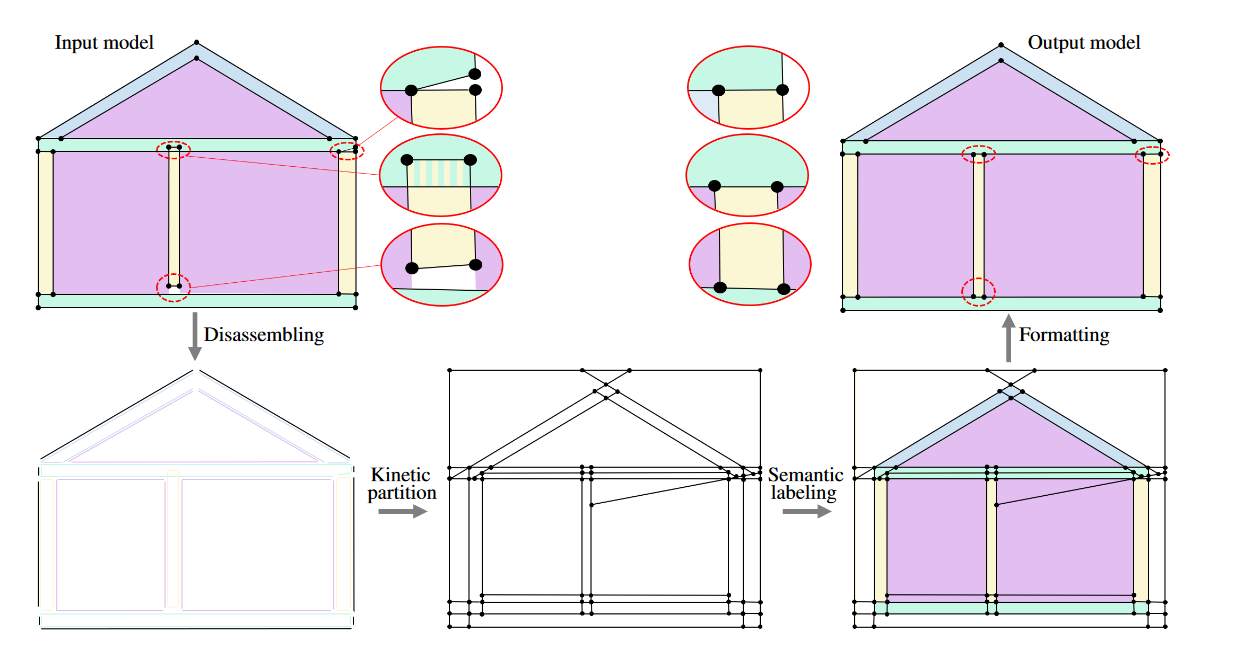
\includegraphics[scale = 0.37]{../../images/example_algorithm_2.png}
\end{frame}
\begin{frame}[plain]{watertight urban model}
    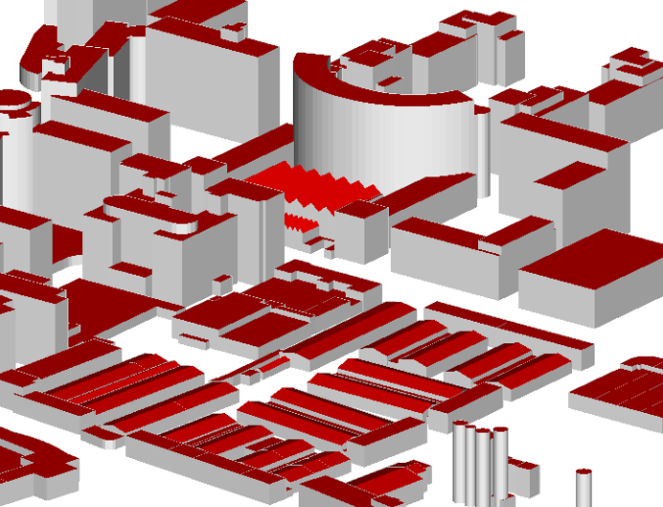
\includegraphics[scale = 0.60]{../../images/example_algorithm_3.png}
\end{frame}

\section{Tools}
\begin{frame}{Tools}
    
    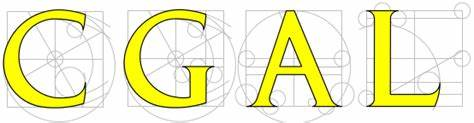
\includegraphics[scale = 0.2]{../../images/CGAL_logo.png}
    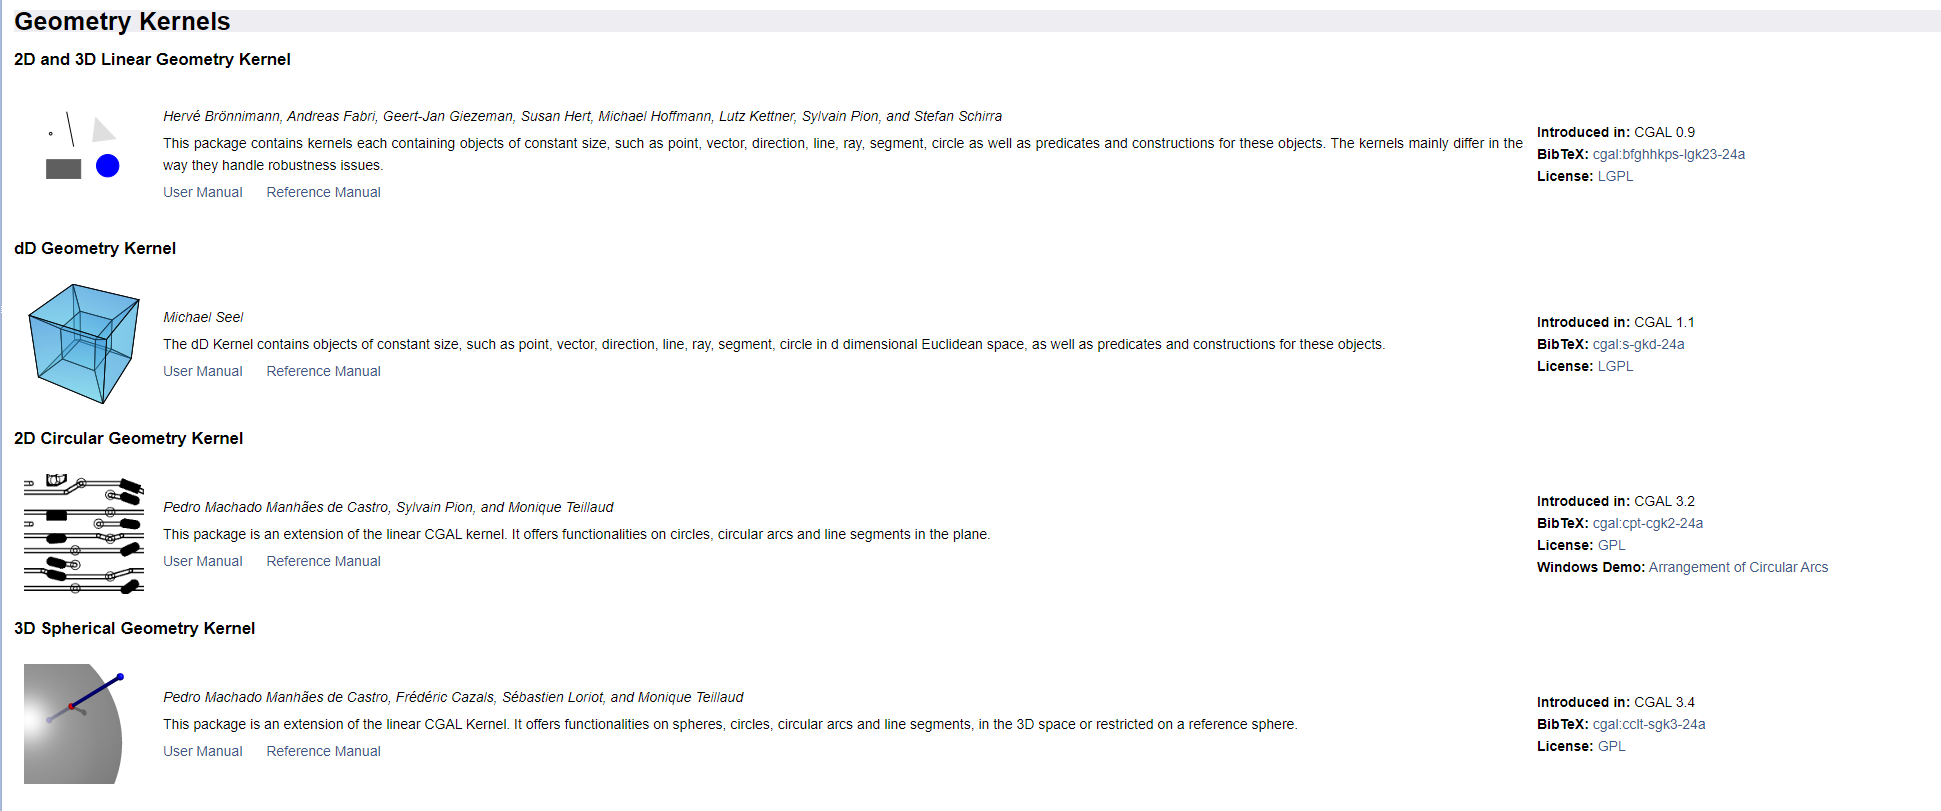
\includegraphics[scale =   0.3 ]{../../images/exemple.png}

\end{frame}



\begin{frame}[plain]{Tools}
    \begin{itemize}
        \item learn how to use CGAL package
        \item learn how to read structure mesh to use it in CGAL code
        \item learn how to use KINETIC package to fill the structure mesh  
    \end{itemize}
\end{frame}
\section{roadmap}

\begin{frame}{roadmap}
    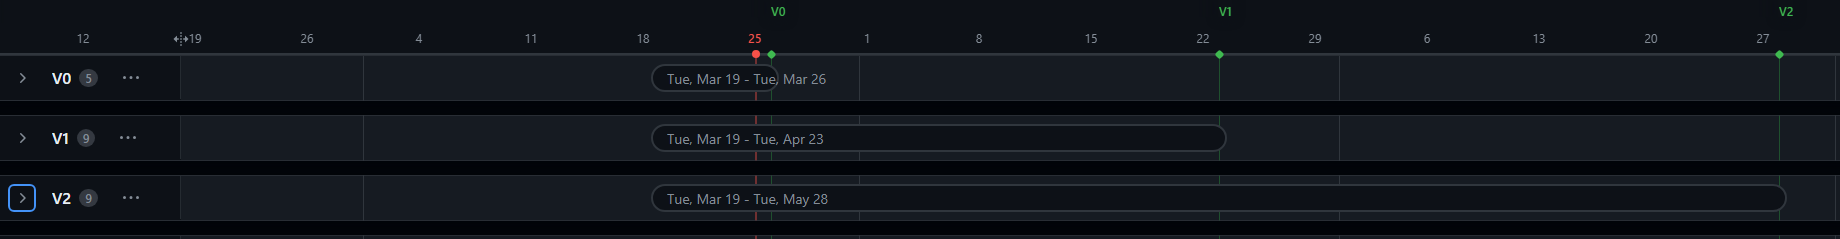
\includegraphics[scale = 0.5]{../../images/roadmap.png}
\end{frame}
\begin{frame}{reference}
    \nocite{*}
    \bibliographystyle{unsrt}
    \bibliography{../../bibliography/v0/report_bib}
\end{frame}

\end{document}